\subsection{No solution}
\draftnote{Arda Baran}
\begin{figure}[H]\centering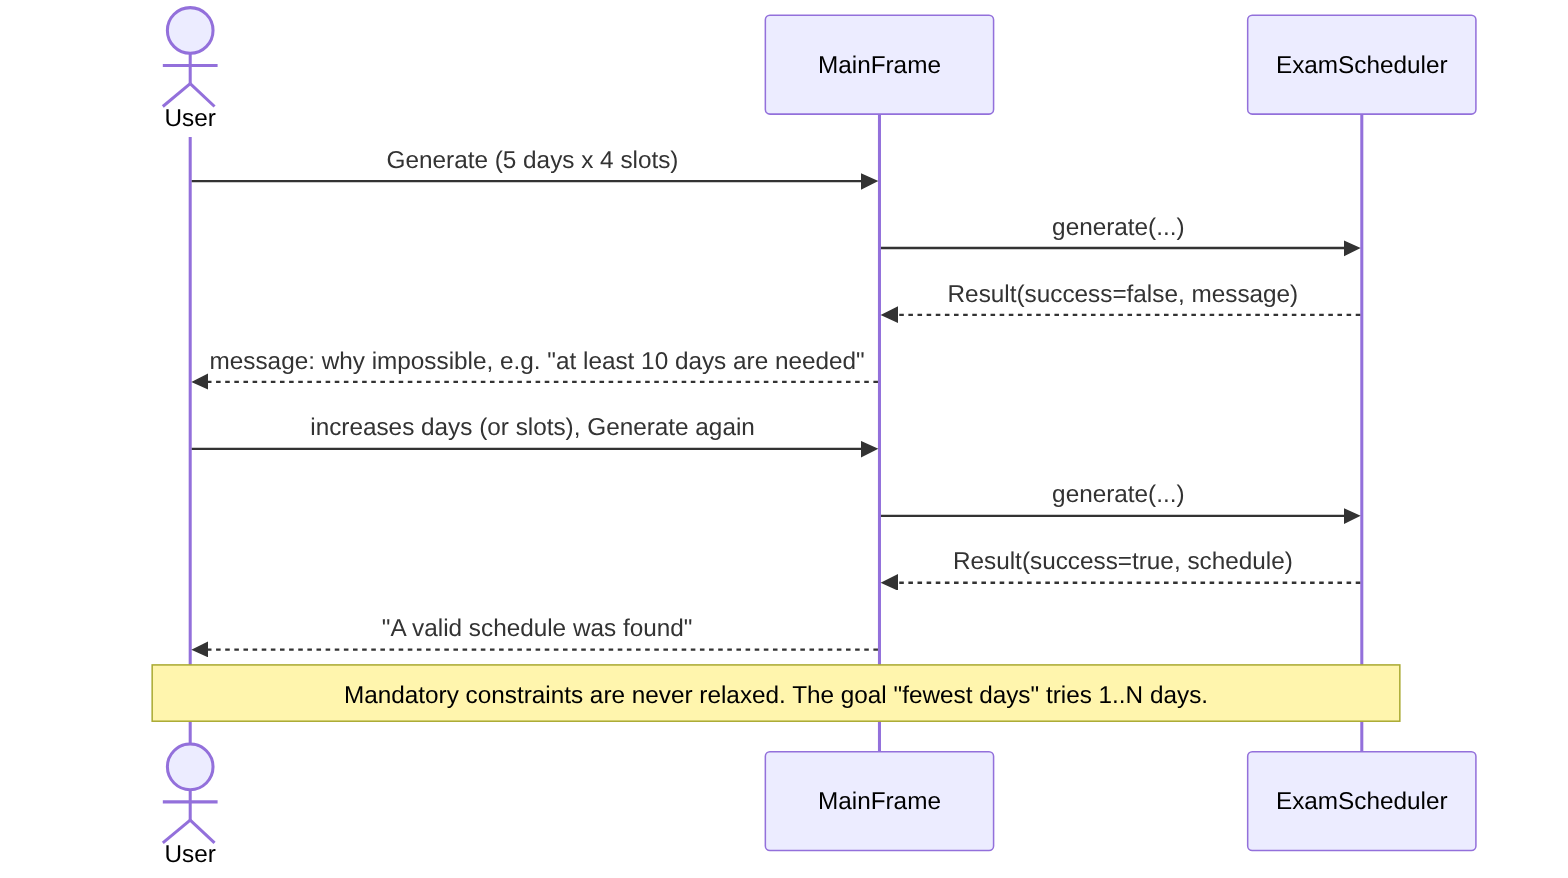
\includegraphics[width=0.8\textwidth]{figures/nosol_flow.png}\caption{No valid schedule for the chosen period.}\end{figure}
Mandatory constraints are never relaxed. Before searching, two necessary conditions are tested: a student with $m$ exams needs at least $\lceil m/2\rceil$ days, and courses that pairwise share students need different slots, of which at most $\lceil s/2\rceil$ fit on one day for $s$ slots per day. If one fails, the message names the reason and the minimum number of days (for the sample data with 5 days and 4 slots: 20 courses share students pairwise, so at least 10 days are needed). If the search runs out of time without proof, the message says no schedule was found in time and suggests more days. In both cases the user increases the days or slots and generates again; nothing is changed.
